% 《博弈论与强化学习》算法实战报告 —— 按课程模板（课程设计报告模板（算法实战）.docx）排版
% 编译：XeLaTeX（Overleaf：Menu → Compiler 选 XeLaTeX）
\documentclass[a4paper,zihao=5,fontset=fandol,UTF8]{ctexart}

% ---------- 版面：与模板一致 ----------
% A4；左右 3.175 cm，上下 2.54 cm；页眉一条横线
\usepackage[a4paper,left=3.175cm,right=3.175cm,top=2.54cm,bottom=2.54cm,headheight=14pt]{geometry}
\usepackage{fontspec}
% 模板西文是 Times New Roman，这里用同款字形的 TeX Gyre Termes（TeX Live 自带）
\setmainfont{texgyretermes}[Extension=.otf,UprightFont=*-regular,BoldFont=*-bold,ItalicFont=*-italic,BoldItalicFont=*-bolditalic]
\setsansfont{texgyreheros}[Extension=.otf,UprightFont=*-regular,BoldFont=*-bold,ItalicFont=*-italic,BoldItalicFont=*-bolditalic]

\usepackage{fancyhdr}
\pagestyle{fancy}
\fancyhf{}
\renewcommand{\headrulewidth}{0.6pt}
\cfoot{\small\thepage}
\fancypagestyle{cover}{\fancyhf{}\renewcommand{\headrulewidth}{0.6pt}}

% 正文：宋体五号，1.2 倍行距（Word 的 1.2 倍约等于此处 1.25），段前段后 2.5 pt，首行缩进 2 字
\linespread{1.25}
\setlength{\parskip}{2.5pt}

% 标题：一级 15 pt「1.」，二级 14 pt「2.1.」，三级 12 pt「2.1.1.」，均加粗
\ctexset{
  section = {format=\fontsize{15pt}{19.5pt}\selectfont\bfseries\heiti\raggedright, name={,.}, number=\arabic{section},
             aftername=\enspace, beforeskip=12pt, afterskip=6pt},
  subsection = {format=\fontsize{14pt}{18.2pt}\selectfont\bfseries\heiti\raggedright, name={,.}, aftername=\enspace,
                beforeskip=8pt, afterskip=4pt, indent=1.5em},
  subsubsection = {format=\fontsize{12pt}{15.6pt}\selectfont\bfseries\heiti\raggedright, name={,.}, aftername=\enspace,
                   beforeskip=6pt, afterskip=3pt, indent=3em},
  figurename = 图, tablename = 表,
}
\renewcommand{\thesubsection}{\thesection.\arabic{subsection}}
\renewcommand{\thesubsubsection}{\thesubsection.\arabic{subsubsection}}

\usepackage{graphicx}
\graphicspath{{figures/}}
\usepackage{booktabs,multirow,array,tabularx}
\usepackage{amsmath,amssymb,bm}
\usepackage[font=small,labelsep=quad,justification=justified,singlelinecheck=true]{caption}
% 表题放在表的上方、居中；图题放在图的下方，一行放得下时居中，多行时两端对齐
\captionsetup[table]{justification=centering,position=top}
\usepackage{enumitem}
% 少量保留的列表：编号与正文首行缩进对齐
\setlist{nosep}
\setlist[enumerate]{label=（\arabic*）,leftmargin=*,labelindent=2em,labelsep=0.2em}
\setlist[itemize]{leftmargin=*,labelindent=2em,labelsep=0.5em}
\usepackage{xcolor}
\usepackage[hidelinks]{hyperref}
\usepackage{float}

% 浮动体：多放图、少留白；只放图的页面从顶部排起，不居中
\renewcommand{\topfraction}{0.9}
\renewcommand{\bottomfraction}{0.6}
\renewcommand{\textfraction}{0.1}
\renewcommand{\floatpagefraction}{0.75}
\setcounter{topnumber}{3}
\setcounter{totalnumber}{4}
\makeatletter
\setlength{\@fptop}{0pt}
\setlength{\@fpsep}{18pt}
\setlength{\@fpbot}{0pt plus 1fil}
\makeatother
\setlength{\textfloatsep}{10pt plus 2pt minus 2pt}

% 图注的第一句话是结论（Nature 图注写法）
\newcommand{\figlead}[1]{\textbf{#1}}

\begin{document}

% =====================================================================
% 封面（照模板）
% =====================================================================
\thispagestyle{cover}
\begin{center}
\vspace*{0.6cm}
{\fontsize{16pt}{24pt}\selectfont\bfseries\heiti 上海大学\ 2026\ \textasciitilde\ 2027\ 学年\ 秋季学期}\\[14pt]
{\fontsize{18pt}{27pt}\selectfont\bfseries\heiti \underline{《博弈论与强化学习》}\quad 算法实战报告}
\end{center}
\vspace{3.2cm}
{\fontsize{14pt}{30pt}\selectfont\heiti
\hspace*{2.6cm}\begin{tabular}{@{}l@{\,}l@{}}
课程设计题目: & \underline{\makebox[7.4cm][l]{\songti 上大校园猫捉老鼠：躲还是跑？}}\\[6pt]
姓名: & \underline{\makebox[5.6cm][l]{\songti 刘明洋}}\\[6pt]
学号: & \underline{\makebox[5.6cm][l]{\songti 24121874}}\\[6pt]
贡献度（百分比）: & \underline{\makebox[2.6cm][l]{\songti 100\%}}\\
\end{tabular}}

\vspace{0.9cm}
{\fontsize{12pt}{16pt}\selectfont\heiti 评分细则:}\par\vspace{4pt}
\noindent\hspace*{-0.45cm}{\fontsize{12pt}{16pt}\selectfont
\renewcommand{\arraystretch}{1.6}\setlength{\tabcolsep}{3pt}
\begin{tabular}{|>{\centering\arraybackslash}m{2.1cm}|>{\centering\arraybackslash}m{2.6cm}|>{\centering\arraybackslash}m{2.1cm}|>{\centering\arraybackslash}m{2.1cm}|>{\centering\arraybackslash}m{2.1cm}|>{\centering\arraybackslash}m{2.1cm}|}
\hline
{\heiti 格式规范}\newline（10\%） & {\heiti 选题创新性}\newline（20\%） & {\heiti 算法实现}\newline（30\%） & {\heiti 实验分析}\newline（20\%） & {\heiti 总结思考}\newline（20\%） & {\heiti 总成绩}\newline（100\%）\\
\hline
 & & & & & \\[16pt]
\hline
\end{tabular}}

\vspace{6pt}
{\fontsize{12pt}{16pt}\selectfont\heiti 课程报告评语:}

\vfill
{\fontsize{12pt}{16pt}\selectfont\heiti 任课教师: \underline{\makebox[3cm]{}}\hfill 评阅日期: \underline{\makebox[2.6cm]{}}}
\vspace{1.5cm}
\newpage

% =====================================================================
% 题目、摘要、关键词
% =====================================================================
\begin{center}
{\fontsize{22pt}{30pt}\selectfont\bfseries\heiti 上大校园猫捉老鼠：躲还是跑？}\\[6pt]
{\fontsize{12pt}{16pt}\selectfont\heiti 真实地图上的多智能体追逃博弈与双方共同强化学习}
\end{center}
\vspace{4pt}

\noindent{\heiti\bfseries 摘要：}%
本文以上海大学宝山校区一次 30 人猫捉老鼠为背景，用 OpenStreetMap 地图把游戏建模为“被抓即转化”的部分可观测随机博弈，结合脚本策略、模仿模型和猫鼠共同强化学习进行分析。结果表明：躲比跑多活约 5.8 分钟，优势主要来自藏身处的隐蔽性；只参照一个同伴时，躲的比例上升很慢；AI 老鼠学到的是针对训练对手的对策；团队平分奖励使猫变弱，奖励要落到在场的猫身上才有效。

\vspace{4pt}
\noindent{\heiti\bfseries 关键词：}追逃博弈；演化博弈；多智能体强化学习；部分可观测随机博弈；奖励结构

\vspace{8pt}

% =====================================================================
\section{引言}
% =====================================================================
本课程设计的题目来自一场真实的线下游戏。上海大学逐浪徒步社团在宝山校区 A–G 楼一带（含 AJ–GJ 楼）组织了一次 30 人的猫捉老鼠：开局 10 只猫、20 只老鼠，碰一下就算抓到，没有安全区；被抓的老鼠立刻变成猫，所有人都知道谁变了。游戏分上下两轮，每轮 30 分钟，开局时所有人在 C、D、CJ、DJ 四栋楼之间的空地集合。活动范围只限楼外的平地，不能进教学楼，因为当时楼里还在上课，而且楼里地形复杂，容易受伤。抓得最多的猫和活得最久的老鼠各有奖励。笔者在第一轮担任老鼠。

玩下来有三条直观经验。第一，活得最久的老鼠都是\textbf{躲}出来的：有人躲在灌木丛里，有人躲在空调外机和教学楼外墙之间的夹缝里。躲在夹缝里的那位一直到最后都没有被抓到，成了这一轮的“鼠王”。第二，猫有时几只一起围一只老鼠，有时一只追一只，也有一只猫追好几只、结果被分头甩开。第三，晚上有夜跑的路人，老鼠常把他们错认成猫，吓一跳。

这些经验背后有几个博弈问题。躲和跑哪个更好，取决于什么条件？一个只想多活一会儿的老鼠，会不会自己学会躲？“抓得最多的猫有奖”是一种个人激励，猫之间既要合作围捕，又在争抢功劳，奖励规则会不会改变猫之间的合作？还有，游戏有上下两轮：第一轮跑的人如果看到躲的人活得更久，第二轮会不会改成躲？反过来，会不会有人从躲改成跑？据此，本文提出五个研究问题：

\begin{enumerate}
  \item \textbf{机制（RQ1）}：在这片校园里，“躲比跑活得久”还成立吗？靠的是“站着不动不显眼”，还是“藏身处不显眼”？
  \item \textbf{最好的藏身点（RQ2）}：灌木丛和夹缝哪个更好，和“鼠王躲在夹缝里”的实战经验一致吗？
  \item \textbf{上下两轮之间的转化（RQ3）}：看到第一轮的结果后，老鼠会从跑转向躲吗？会出现从躲转向跑的反方向转化吗？
  \item \textbf{老鼠的学习（RQ4）}：只奖励“活得久”、和猫一起学习的 AI 老鼠，会不会自己学会躲？如果藏身处不再有隐蔽优势，它会不会改成跑？它学到的本领换个对手还管用吗？
  \item \textbf{猫的学习（RQ5）}：不把围捕写进规则，猫能不能自己学会？个人奖励和团队奖励下，猫的强弱和围捕有什么不同？
\end{enumerate}

% =====================================================================
\section{相关工作}
% =====================================================================
表~\ref{tab:related} 先给出相关工作与本文的对应关系，下面再逐类说明。

\begin{table}[htbp]
  \centering\small
  \caption{相关工作与本文的对应关系}
  \label{tab:related}
  \renewcommand{\arraystretch}{1.25}
  \begin{tabularx}{\textwidth}{@{}p{3.1cm}X X@{}}
    \toprule
    文献 & 研究的问题 & 本文借鉴或对照的地方\\
    \midrule
    搜索博弈\cite{alpern2003,chung2011} & 藏的一方选位置，找的一方选搜索路线 & 发现模型（第~\ref{sec:detect} 节）；猫的巡逻和搜索策略\\
    多智能体捉迷藏\cite{baker2020} & 藏者和找者一起训练，会自己学出新策略 & 猫和老鼠一起训练，看老鼠会不会自己学会躲（RQ4）\\
    PPO 与 GAE\cite{schulman2017ppo,schulman2016gae,yu2022mappo} & 稳定的策略梯度训练方法 & 本文的训练算法（第~\ref{sec:obs} 节）\\
    追捕中的奖励结构\cite{grupen2022,leibo2017} & 个人奖励和共享奖励下，追捕者会不会合作 & 猫的个人奖励与团队奖励对比（RQ5）\\
    演化博弈与模仿\cite{taylor1978,szabo1998,traulsen2006} & 人们看到别人的收益后怎样改策略 & 上下两轮之间的策略转化（RQ3）\\
    传染过程\cite{kermack1927} & 接触后“被感染”的人数怎样增长 & 被抓的老鼠变成猫，猫越来越多\\
    \bottomrule
  \end{tabularx}
\end{table}

\subsection{捉迷藏与搜索博弈}
捉迷藏在博弈论里叫搜索博弈：藏的一方选一个位置，找的一方选一条搜索路线，双方都希望对方猜不中\cite{alpern2003}。机器人领域把它和追捕问题合在一起研究，并指出视线被障碍挡住时，追捕会先变成“找人”，找到以后才是“追人”\cite{chung2011}。本文的游戏正是如此：老鼠被发现之前，是猫在找；被发现之后，才是猫在追。“躲”的作用是让老鼠尽量停留在“找”的阶段。本文用一个发现模型（第~\ref{sec:detect} 节）来描述“找”的难度，用猫的巡逻和搜索策略来描述“找”的方式。

\subsection{多智能体强化学习中的捉迷藏}
与本文最接近的是 OpenAI 的捉迷藏实验\cite{baker2020}：藏者和找者用强化学习一起训练，双方先后学出了堵门、搬箱子等策略，而这些策略都没有写进规则。本文借用这种“双方一起学”的做法，看只奖励“活得久”的老鼠会不会自己学会躲。训练算法采用近端策略优化（PPO）\cite{schulman2017ppo} 和广义优势估计（GAE）\cite{schulman2016gae}；同一阵营的个体共用一套网络参数，这种做法在多智能体任务中很常用\cite{yu2022mappo}。需要说明的是，本文的价值网络只用每个人自己的观测，属于“按阵营共享参数的独立 PPO”，不是集中式训练。

\subsection{奖励结构与合作}
Grupen 等人研究了多只追捕者抓一只逃跑者的任务\cite{grupen2022}：追捕者只拿自己的奖励时，倾向于各自贪心地追；改成共享奖励后，更容易形成包抄。他们也指出，共享奖励下抓捕数会集中在少数个体身上，这可能是分工（有人负责堵、有人负责抓），不一定是偷懒。Leibo 等人则说明，个体利益与集体利益的冲突会出现在多步决策中\cite{leibo2017}。本文的猫既要合作围捕，又在比谁抓得多，正好可以检验奖励方式对合作的影响。

\subsection{演化博弈与模仿}
演化博弈研究的是策略怎样在人群中传播：收益高的策略会被更多人采用，这一过程可以用复制者动态描述\cite{taylor1978}。在个体层面，常用的模型是“两两比较”：每个人看一个同伴，同伴收益比自己高时，以一定概率改用同伴的策略，这个概率用费米函数刻画，下文称为费米模仿规则\cite{szabo1998,traulsen2006}。本文用它来回答 RQ3：第一轮结束后，看到别人收益的老鼠会怎样改策略。

\subsection{传染式的转化}
被抓的老鼠变成猫，类似传染病里“易感者接触感染者后被感染”的 SI 过程\cite{kermack1927}：猫越多，剩下的老鼠越危险。这里只是类比，本文的接触过程由移动、视线和策略决定，并没有用流行病方程建模。

% =====================================================================
\section{算法设计}
% =====================================================================
\subsection{环境：基于 OpenStreetMap 的 A–G 楼地图}
地图来自 OpenStreetMap（OSM）\cite{osm}。OSM 是二维地图，记录的是建筑轮廓、道路、林地等平面要素，没有地形起伏，也没有完整的建筑高度，因此本文把场地当作平面，把楼当作完全挡住视线的墙。笔者用 Overpass 接口下载了宝山校区的全部要素（共 19655 个），截取 A–GJ 楼外扩 25 m 的区域，共 418 m × 526 m，按 0.5 m 一格栅格化成 836 × 1053 的格子图（图~\ref{fig:env}a）。

每个格子属于五类之一：平地（路、广场、草坪，共 15.4 万 m²）可以正常行走；教学楼（4.9 万 m²）不能进入，并且挡住视线；灌木丛（1.5 万 m²）取自 OSM 的林地和行道树，可以进入，但只能以 0.8 m/s 慢慢挪；空调外机夹缝（391 m²）；其余是场地外，不能去。下载的 OSM 数据中没有任何与空调外机有关的标签，也就是说 OSM 并没有采集空调外机的位置，因此本文只能按固定随机种子沿 A–GJ 楼外墙放置 235 台空调外机，平均每 14 m 一台，每台和外墙之间留出 2 m 长、1 m 深的夹缝。这一部分是合成的，不代表实际位置。

开局集合点取 C、D、CJ、DJ 四栋楼中心的平均位置附近最近的空地，与实际游戏一致；所有人在集合点周围 30 m × 30 m 范围内的空地上随机出生。寻路方面，笔者在 4 m 的粗格上（11269 个结点）用 Dijkstra 算法预先算好任意两点之间的下一跳。智能体每一步先检查到目标的直线是否通畅，通畅就直走，否则沿最短路绕楼走。

\begin{figure}[htbp]
  \centering
  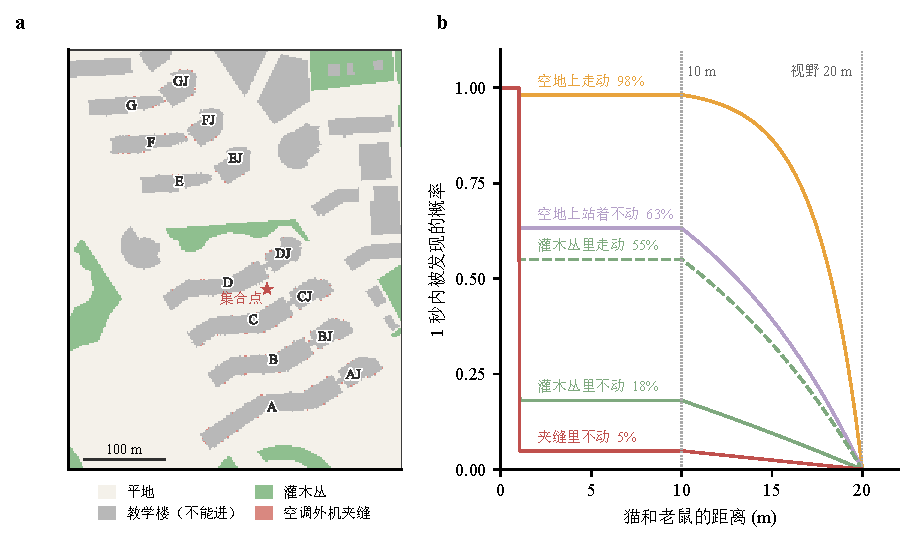
\includegraphics[width=\textwidth]{fig0_environment.pdf}
  \caption{\figlead{场地取自 OpenStreetMap 的 A–G 楼一带，“藏在哪里、动不动”决定了被发现的快慢。}
  \textbf{a}，栅格化后的场地（0.5 m 一格）。红点是沿外墙放置的空调外机夹缝（合成）；红星是开局集合点，位于 C、D、CJ、DJ 四栋楼之间。
  \textbf{b}，一只猫在不同距离上看着老鼠时，老鼠 1 秒内被发现的概率。曲线旁的百分比是 5 m 处的数值。10 m 以内速率不变，之后线性下降，到 20 m 降为 0；1 m 以内必定被发现。}
  \label{fig:env}
\end{figure}

\subsection{博弈建模：被抓即转化的部分可观测随机博弈}
本文把一轮游戏写成一个 30 名玩家、有限时域的部分可观测随机博弈（POSG）
\begin{equation*}
\mathcal{G}=\langle \mathcal{N}, \mathcal{S}, \rho_0, \{\mathcal{A}_i\}, \{\mathcal{O}_i\}, O, P, \{r_i\}, T\rangle .
\end{equation*}
玩家集合 $\mathcal{N}$ 为 30 人。状态 $s_t$ 包括所有人的位置、速度、体力、身份（猫或老鼠），夜跑路人的位置和目的地，以及每只猫对每只老鼠“是否正在盯住”的标记。初始分布 $\rho_0$ 是：10 只猫、20 只老鼠在集合点附近随机出生。观测函数 $O$ 把全局状态映射为每个人的观测 $o_i\in\mathcal{O}_i$，由第~\ref{sec:detect} 节的发现模型定义：每个人只看得到自己的状态和视线内、20 m 以内的人，具体构成见表~\ref{tab:obs}。时域 $T$ 为 30 分钟（3600 步，步长 $\Delta t=0.5$ s），老鼠全部被抓时这一局提前结束。

状态转移中最特别的是身份转移：老鼠 $i$ 与猫 $j$ 的距离小于 0.6 m 即被抓，$i$ 的身份立刻变为猫，同时记 $j$ 抓到一只。因此玩家总数不变，但两个阵营的人数随时间变化，一名玩家在一轮中可能先当老鼠、后当猫。本文把这两个阶段分开处理：老鼠阶段的目标是活得久，猫阶段的目标是多抓。开局猫原地数 60 秒。运动方面，冲刺 4 m/s、慢跑 2.5 m/s、走 1.5 m/s，灌木丛和夹缝里最快 0.8 m/s；冲刺最多持续 20 s，走路或站着时恢复。碰撞检测把每步分成 4 个子步，撞墙后沿墙滑动。

这是一个一般和博弈：老鼠的存活收益和猫的抓捕收益加起来并不是常数，双方收益也不互为相反数。老鼠之间没有直接冲突，但任何一只老鼠被抓，都会让其余老鼠面对的猫多一只。

\subsection{发现模型与反事实对照}
\label{sec:detect}
猫 $j$ 能“看到”老鼠 $i$ 的前提是两人之间视线不被楼挡住，且距离 $d<R=20$ m（晚上路灯下的视野）。在这个前提下，每一步以概率 $1-e^{-\lambda\Delta t}$ 发现对方，速率为
\begin{equation}
\lambda = \lambda_0 \cdot g(d) \cdot f_{\text{静}}^{\,\mathbb{1}[\text{静止}]} \cdot f_{\text{地形}}, \qquad
g(d)=\min\!\left(1,\ 2\left(1-\tfrac{d}{R}\right)\right)_{+},
\end{equation}
其中 $\lambda_0=4\ \text{s}^{-1}$。速度低于 0.3 m/s 视为静止，$f_{\text{静}}=0.25$；在灌木丛里 $f_{\text{地形}}=0.2$，在夹缝里 $f_{\text{地形}}=0.05$，在平地上为 1。1 m 以内必定发现。一旦被发现，猫会一直盯住目标，直到视线被楼挡住或距离超过 20 m。图~\ref{fig:env}b 给出了各状态下 1 秒内被发现的概率：在 5 m 处，空地上走动是 98\%，夹缝里不动只有 5\%。老鼠这一侧，6 个夜跑路人在路上慢跑，老鼠在 5 m 以外认不出路人是不是猫，所以远处的路人和猫一样会引发逃跑。

这些系数是笔者根据游戏体验设定的，不是测量值。现实中，藏在夹缝里、站着不动当然更难被发现；本文并不怀疑这一点。实验中把某个系数改成 1（即“这个因素不再带来隐蔽优势”），是一种\textbf{反事实对照}：如果改掉某个因素之后，躲的优势就消失了，就说明在这个模型里，躲的优势正是由这个因素带来的；如果改掉之后优势还在，说明还有别的原因（例如藏身点的位置、路线）。这样做的目的是找出“躲为什么有效”，而不是判断现实中藏身处是否更隐蔽。本文分别做三组对照：只取消静止的优势（$f_{\text{静}}=1$）、只取消地形的优势（$f_{\text{灌木}}=f_{\text{夹缝}}=1$）、以及两者都取消。

\subsection{脚本策略}
\label{sec:script}
脚本策略是写好固定规则的猫和老鼠，用来回答 RQ1–RQ3，也作为强化学习的对照。猫的策略分三层：看见老鼠，就按对方速度预判 2 s 后的位置并去拦截；跟丢了，就去最后看见的位置附近搜 30 秒；都没有，就巡逻——全队共享一张 20 m × 20 m 的“多久没人搜过”表，每只猫从 4 个随机候选格中挑最久没搜过的一个去搜。

老鼠有五种策略。\textbf{跑}：慢跑游走，一见到猫（或 5 m 外认不出的路人）就冲刺逃离，逃跑方向从 16 个方向里选，既要远离威胁，又要保证前方 1.5 m 和 3 m 都能走。\textbf{躲}：走到最近的灌木或夹缝藏好不动，猫进入 10 m 才逃，逃完再换一个藏身点，选点时兼顾“离自己近、离威胁远”。\textbf{只躲灌木}和\textbf{只躲夹缝}与之相同，但只选一种藏身点。\textbf{原地不动}：不找掩体，就地站着，猫进入 10 m 才逃。

\subsection{上下两轮之间的策略转化}
\label{sec:imitate}
为回答 RQ3，本文让 20 只老鼠中躲的比例 $x$ 分别取 0、0.25、0.5、0.75、1（其余都跑），每个 $x$ 跑 256 局，得到躲者和跑者各自的收益（30 分钟内的平均存活时间）$\pi_H(x)$ 和 $\pi_R(x)$。在此基础上模拟第一轮结束后的模仿：每只老鼠随机看同一局里的一个同伴，若同伴采用另一种策略，就以概率
\begin{equation}
p = \frac{1}{1+\exp\!\big(-(\pi_{\text{同伴}}-\pi_{\text{自己}})/K\big)}
\end{equation}
改用同伴的策略\cite{szabo1998,traulsen2006}。$K$ 表示“看别人结果时的随机性”：$K$ 越小，越只跟着收益高的人学。$\pi$ 用的是这一局里两人各自的实际存活时间，所以即使躲的平均收益更高，也会有“这一局躲的人运气差、跑的人运气好”的情况，从而出现从躲到跑的反方向转化。本文统计两个方向的转化比例，以及第二轮躲的比例。

\subsection{双方共同训练的 PPO}
\label{sec:obs}
猫和老鼠各用一张网络（两层、每层 256 个单元），同一阵营的所有个体共用参数。老鼠被抓后，下一步起改由猫网络控制。两张网络同时用 PPO 训练，互为对方的环境。两张网络的输入相同，共 218 维（表~\ref{tab:obs}）。

\begin{table}[htbp]
  \centering\small
  \caption{强化学习的观测（每人 218 维）}
  \label{tab:obs}
  \renewcommand{\arraystretch}{1.2}
  \begin{tabularx}{\textwidth}{@{}lcX@{}}
    \toprule
    内容 & 维数 & 说明\\
    \midrule
    自身状态 & 11 & 位置、速度、剩余体力、已用时间、脚下地形、场上猫的比例、自己的身份（被抓后所有人都知道，属于公开信息）\\
    8 个方向到墙的距离 & 8 & 20 m 以内\\
    周围地形 & 147 & 以自己为中心 14 m × 14 m 的 7 × 7 局部图，灌木、夹缝、建筑三个通道\\
    最近 5 个对手 & 25 & 相对位置、速度、是否有效。老鼠：自己看见的猫和认不出的路人（用路人的真实速度）；猫：自己或 30 m 内队友正在盯住的老鼠（相当于喊话报位置）\\
    最近 4 个队友 & 20 & 只包括视线内、20 m 以内的队友\\
    记忆 & 3 & 最后一次看见对手的位置和距今时间\\
    提示 & 4 & 当前藏身目标、巡逻目标的方向\\
    \bottomrule
  \end{tabularx}
\end{table}

老鼠有 27 个动作：停下，8 个方向 × 3 档速度，外加“沿路去最近的藏身点”和“冲刺逃离”两个现成动作。猫有 20 个动作：停下，8 个方向 × 2 档速度，外加“沿路追（带预判）”“去最后看见的地方”“巡逻”三个现成动作。本文没有给猫“包抄”动作，围捕只能通过方向动作和追击动作的配合出现。

老鼠每活一步得 $\Delta t/60$，即每活 1 分钟得 1 分；被抓后，它作为老鼠的轨迹终止。猫的奖励分两组：\textbf{个人奖励}组自己抓到一只得 1 分，是真实游戏“抓得最多的猫有奖”的近似（真实游戏是按名次发奖，这里改成按只计分）；\textbf{团队奖励}组全队每抓到一只，抓捕前已经是猫的每个成员平分 1 分。为了检验“团队奖励的问题出在功劳被稀释”这个猜想，又加了两组：\textbf{混合奖励}取个人奖励和团队奖励各一半；\textbf{按参与分配}把每次抓捕的 1 分只分给抓捕瞬间离受害者 15 m 以内、抓捕前已经是猫的成员（平均每次约 3.4 只）。后者是一种局部共享奖励：它仍然奖励“在场”而不是精确地衡量每只猫的贡献，并不是严格意义上的差分奖励。“按参与分配”和团队奖励相比改了两件事：分到功劳的猫变少了（奖励更集中），而且分到的是在场的猫（奖励与行为挂钩）。为了把这两点分开，再加一组\textbf{随机分配}对照：每次抓捕分给几只猫与“按参与分配”完全相同，但这几只猫是从全体猫中随机抽的，与它在不在场无关（实测只有约四成恰好在场）。

共同训练还有一个已知问题：双方只和对方的\textbf{当前}版本对局，容易学成只能打败这一个对手的对策。为此本文加了\textbf{历史对手池}组（一种基于历史快照的自我对弈）：每 25 轮把双方网络存一份快照；每开一批新局，每方从快照里随机抽 4 份，分给不同的局。一半的局让当前老鼠对历史猫，只训练老鼠；另一半让历史老鼠对当前猫，只训练猫。这样每方实际用到的样本只有普通组的一半，所以历史对手池组训练 600 轮，样本量与普通组的 300 轮大致相同。为了把“对手更多样”和“样本减半、训练轮数加倍”这两个因素分开，另设\textbf{只用最新对手}组：流程完全相同，但快照池只保留最近一份。

抓捕判定在每个移动子步都检查一次距离（一步 0.5 秒分 4 个子步），避免猫和老鼠迎面跑过、在两次检查之间擦身而过却不算抓到。各方的动作只改写自己的状态，例如猫的巡逻动作不会改动老鼠的目标点。

计算优势时，GAE 需要知道下一步还是不是同一张网络在控制这个人。本文为每个人、每一步记录角色掩码 $m_{t+1}$：老鼠在 $t\to t+1$ 之间被抓，则 $m_{t+1}=0$，这一段对老鼠网络而言就是终止；某一局老鼠全部被抓后，这一局也立即终止，不再产生训练样本。记 $d_t$ 为这一步是否终止，则
\begin{equation}
\delta_t = r_t + \gamma\, m_{t+1}\,(1-d_t)\, V(o_{t+1}) - V(o_t),\qquad
\hat A_t = \delta_t + \gamma\lambda\, m_{t+1}\,(1-d_t)\,\hat A_{t+1}.
\end{equation}
训练要最小化的损失是剪切形式的 PPO 目标，加上价值损失和熵正则：
\begin{equation}
\begin{aligned}
L(\theta)={}&-\mathbb{E}_t\!\left[\min\!\big(\rho_t\hat A_t,\ \operatorname{clip}(\rho_t,1-\epsilon,1+\epsilon)\hat A_t\big)\right]\\
&+\tfrac12\,\mathbb{E}_t\!\left[(V_\theta(o_t)-\hat R_t)^2\right]-c_H\,\mathbb{E}_t\!\left[\mathcal H(\pi_\theta(\cdot|o_t))\right],
\end{aligned}
\end{equation}
其中 $\rho_t=\pi_\theta(a_t|o_t)/\pi_{\theta_{\text{old}}}(a_t|o_t)$，价值目标 $\hat R_t=\hat A_t+V_{\theta_{\text{old}}}(o_t)$。超参数见表~\ref{tab:hp}。折扣 $\gamma=0.995$ 对应的“半衰期”约 69 秒，也就是说，网络更看重一两分钟内的生存，对几分钟以后的收益看得较轻。

\begin{table}[htbp]
  \centering\small
  \caption{训练超参数}
  \label{tab:hp}
  \begin{tabular}{@{}ll@{\qquad}ll@{}}
    \toprule
    参数 & 取值 & 参数 & 取值\\
    \midrule
    并行局数 & 64 & 每轮采样步数 & 128 步（64 s）\\
    一局时长 & 30 分钟（3600 步） & 训练轮数 & 300（对手池两组 600）\\
    折扣 $\gamma$ / GAE $\lambda$ & 0.995 / 0.95 & 剪切 $\epsilon$ & 0.2\\
    学习率（Adam） & $3\times10^{-4}$ & 每轮更新 & 4 遍，小批量 16384\\
    熵系数 $c_H$ & 0.01 & 梯度裁剪 & 0.5\\
    训练组 & 8 组（见正文） & 每组训练种子 & 3 个\\
    \bottomrule
  \end{tabular}
\end{table}

\subsection{评价指标}
存活时间指一轮 30 分钟内的平均存活时间，没被抓的老鼠记 30 分钟。同一局里的老鼠面对同一批猫，彼此并不独立，所以本文的置信区间一律\textbf{按局}重采样（2000 次自举，取 95\% 区间）\cite{agarwal2021}；比较两种策略时，用同一局内的配对差。强化学习的结果先按训练种子分别评估（每个种子 64 局，评估用与训练不同的固定随机种子），组均值取各种子均值的平均；置信区间用分层自举，先重抽训练种子，再在种子内重抽局，这样区间同时反映对局的随机性和训练种子之间的差异。只有 3 个种子时，这个区间很宽，也不够精确，所以强化学习部分的比较只作探索性结论。老鼠行为用五类时间占比描述：静止、在灌木丛里、在夹缝里、贴楼 2 m 以内、冲刺，这五类可以重叠，加起来不必是 100\%。

围捕指标在每次抓捕的瞬间计算，只统计抓捕之前就已经是猫的个体：一是受害者 15 m 内有没有至少 2 只猫；二是包围度 $1-\theta_{\max}/2\pi$，其中 $\theta_{\max}$ 是 20 m 内的猫相对受害者的最大角度空缺，猫全在同一侧时接近 0，四面包围时接近 1。这两个量描述的是抓捕瞬间猫的空间聚集，并不直接等于合作，因为场上猫越多，它们自然越容易聚在一起。猫之间的分配用开局 10 只猫的抓捕数基尼系数描述。基尼系数衡量分配的不均匀程度：0 表示每只猫抓到的数量完全相同，越接近 1 表示抓捕越集中在少数几只猫身上。


% =====================================================================
\section{实验结果与分析}
% =====================================================================
\subsection{实验环境与设置}
环境用 PyTorch 在 GPU 上批量并行实现，所有人的感知、移动、碰撞和抓捕都写成张量运算，在一块 NVIDIA RTX 4070 Laptop GPU（8 GB）上运行，软件环境为 Python 3.12 与 PyTorch。

实验分四部分，一轮都是 30 分钟。脚本策略实验每种条件跑 256 局，同一局里 20 只老鼠按五种策略各 4 只分配，用局内配对比较。“哪里最好躲”实验让每只老鼠开局被分到全图随机的一个藏身点，共 2 × 256 局。上下两轮转化实验对 5 种躲的比例各跑 256 局。共同训练实验有八组：猫的五种奖励（个人、团队、混合、按参与分配、随机分配）、隐蔽无优势、历史对手池、只用最新对手。每组 3 个种子，普通组训练 300 轮（每个约 27 分钟），对手池两组训练 600 轮（每个约 50 分钟），之后每个种子用 64 局做交叉评估。在上真实地图之前，笔者先在 50 m × 50 m 的抽象小场地上做了一轮机制探针，结果见第~\ref{sec:res-probe} 节。

\subsection{先导实验：小场地上，躲赢在“动起来更显眼”}
\label{sec:res-probe}
小场地上扫了四个因素：掩体多少、体力是否有限、静止时是否更难被发现、老鼠知不知道谁刚变成猫，每种条件跑 1024 局，一局 300 s。如图~\ref{fig:probe}a，只要“动静一样显眼”，躲就不比跑好，体力无限时在空地上跑反而多活 10 s；一旦静止时更难被发现，躲在每种掩体数量下都赢。体力限制的作用比预想的小。小场地上没有灌木和夹缝这样的“难被看见的地形”，所以这里只检验了“静止”这一项。

\begin{figure}[htbp]
  \centering
  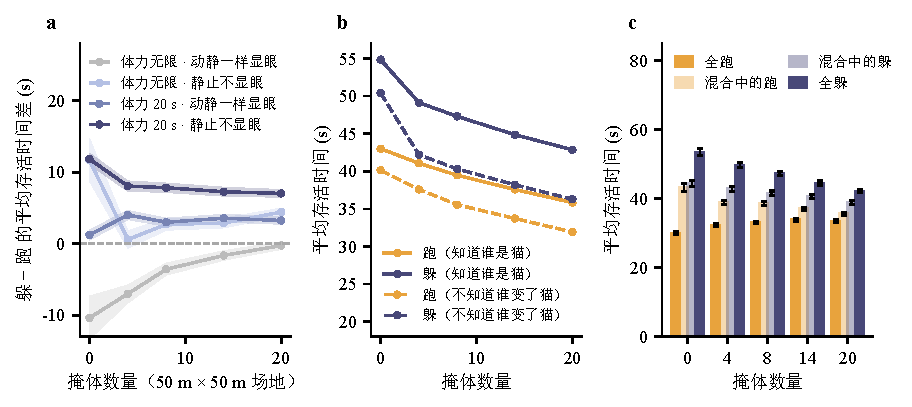
\includegraphics[width=\textwidth]{fig1_hide_vs_run.pdf}
  \caption{\figlead{在 50 m 小场地上，只有“动起来更显眼”时，躲才稳定地比跑活得久。}
  \textbf{a}，同一局里躲的老鼠减去跑的老鼠的平均存活时间差，按四种“体力 × 显眼度”组合画出。阴影为 95\% 自举区间，每点 1024 局。
  \textbf{b}，老鼠不知道谁刚变成猫时（虚线），躲的优势缩小。
  \textbf{c}，体力 20 s、动静一样显眼时，全跑、全躲和混合（各半）三种群体下的人均存活。误差棒为 95\% 自举区间。}
  \label{fig:probe}
\end{figure}

笔者也在小场地上训练了只有老鼠学习的 PPO（猫是脚本，每种条件 3 个种子，图~\ref{fig:probe-ppo}）。在真实条件下，AI 老鼠活 51–56 s，比脚本躲（50 s）和脚本跑（39 s）都久。它学到的不是“躲到掩体后面”：只有 6\% 的时间贴着掩体，却有 70\% 的时间贴着墙。背靠墙，危险只会从半边来。

\begin{figure}[htbp]
  \centering
  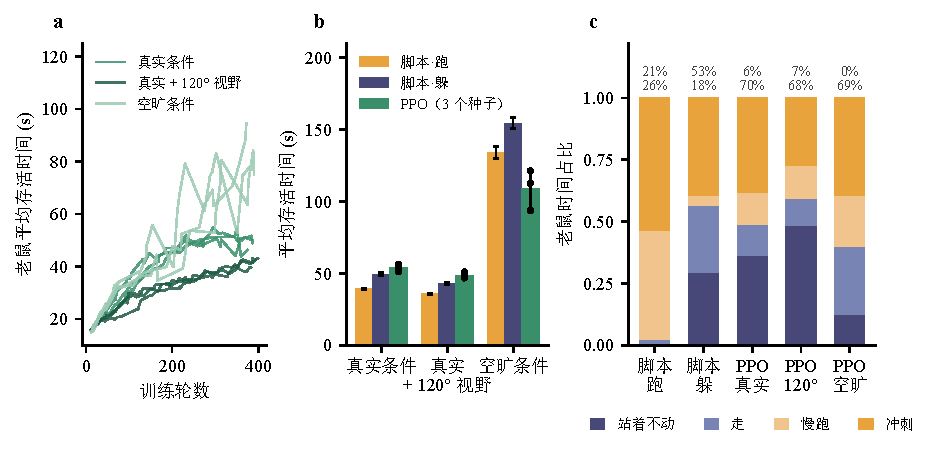
\includegraphics[width=\textwidth]{fig2_ppo_behavior.pdf}
  \caption{\figlead{小场地上的 AI 老鼠学会了“背靠墙站着不动”，而不是躲到掩体后面。}
  \textbf{a}，训练曲线，每条线一个随机种子。
  \textbf{b}，评估时的平均存活时间，评估用训练时没见过的地图布局。脚本策略的误差棒为 95\% 自举区间；PPO 的黑点是各种子的结果，误差棒为 3 个种子的最小值到最大值。
  \textbf{c}，老鼠时间分配。柱顶两行数字分别是贴掩体、贴墙的时间占比。}
  \label{fig:probe-ppo}
\end{figure}

\subsection{真实地图上：躲比跑活得久，优势主要来自藏身处本身}
\label{sec:res-campus}
图~\ref{fig:campus}a 是基准条件下五种策略的存活曲线，表~\ref{tab:campus} 给出各条件下的平均存活和以跑为对照的局内配对差。基准条件下，就近选灌木或夹缝的“躲”平均活 11.2 分钟，比跑多 5.8 分钟（95\% 区间 [4.9, 6.7]）；只躲夹缝与它几乎一样，11.1 分钟；原地不动 8.5 分钟，只躲灌木 6.3 分钟，也都好过跑（5.4 分钟）。“躲”和“只躲夹缝”分别有 28\% 和 27\% 的老鼠撑满了 30 分钟，跑的老鼠只有 3\%。所以 RQ1 的第一问得到了肯定的回答：在这片校园里，躲确实比跑活得久。

\begin{figure}[htbp]
  \centering
  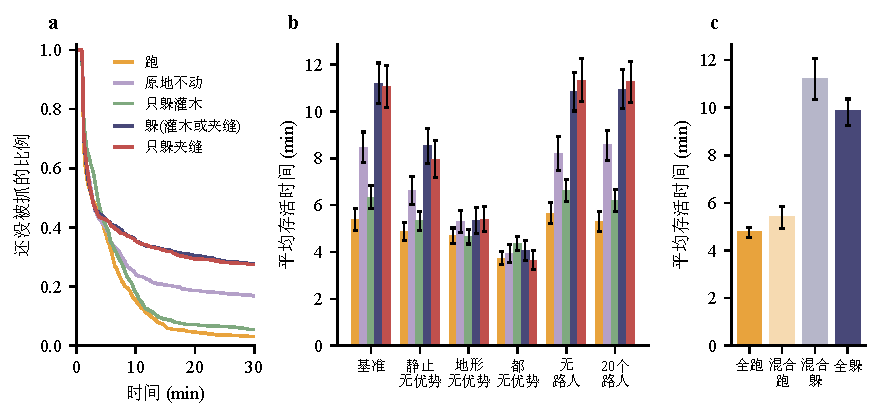
\includegraphics[width=\textwidth]{fig3_campus_hide_vs_run.pdf}
  \caption{\figlead{在真实地图上躲比跑活得久；取消藏身处的隐蔽优势后，躲的优势大部分消失。}
  \textbf{a}，基准条件下五种策略的存活曲线（每种策略 1024 只老鼠，一轮 30 分钟）。
  \textbf{b}，六种条件下的平均存活时间：基准；静止无优势（$f_{\text{静}}=1$）；地形无优势（$f_{\text{灌木}}=f_{\text{夹缝}}=1$）；两者都无优势；无夜跑路人；20 个路人。颜色同 \textbf{a}，误差棒为按局自举的 95\% 区间，每种条件 256 局。
  \textbf{c}，全跑、全躲两种同质群体与混合群体的对比（每组 256 局）。浅色柱是混合群体中该策略老鼠的人均存活。}
  \label{fig:campus}
\end{figure}

\begin{table}[htbp]
  \centering\small
  \caption{真实地图上各策略的平均存活（分钟）与“该策略 − 跑”的局内配对差。方括号是按局自举的 95\% 区间，每格 256 局 × 4 只老鼠。}
  \label{tab:campus}
  \footnotesize\setlength{\tabcolsep}{2.5pt}
  \begin{tabular}{@{}lccccc@{}}
    \toprule
    条件 & 跑 & 原地不动 & 只躲灌木 & 躲（灌木或夹缝） & 只躲夹缝\\
    \midrule
    % 以下各行由 catmouse/make_tables.py 生成
    基准 & 5.4 & 8.5（+3.1 [2.3, 3.9]） & 6.3（+1.0 [0.3, 1.7]） & 11.2（+5.8 [4.9, 6.7]） & 11.1（+5.7 [4.8, 6.6]）\\
    静止无优势 & 4.9 & 6.6（+1.7 [1.1, 2.4]） & 5.3（+0.4 [$-$0.1, 1.0]） & 8.5（+3.7 [2.8, 4.5]） & 7.9（+3.0 [2.3, 3.9]）\\
    地形无优势 & 4.7 & 5.3（+0.6 [0.0, 1.2]） & 4.6（$-$0.0 [$-$0.5, 0.4]） & 5.3（+0.6 [0.0, 1.2]） & 5.4（+0.7 [0.1, 1.3]）\\
    两者都无优势 & 3.7 & 3.9（+0.2 [$-$0.3, 0.6]） & 4.3（+0.6 [0.2, 1.0]） & 4.1（+0.3 [$-$0.2, 0.8]） & 3.6（$-$0.1 [$-$0.6, 0.4]）\\
    无夜跑路人 & 5.7 & 8.2（+2.6 [1.8, 3.3]） & 6.6（+1.0 [0.4, 1.6]） & 10.8（+5.2 [4.3, 6.1]） & 11.3（+5.7 [4.7, 6.7]）\\
    20 个路人 & 5.3 & 8.6（+3.3 [2.5, 4.0]） & 6.2（+0.9 [0.3, 1.5]） & 10.9（+5.6 [4.8, 6.5]） & 11.3（+6.0 [5.1, 6.9]）\\
    \bottomrule
  \end{tabular}
\end{table}

第二问是：躲的优势靠的是什么？这里要用到第~\ref{sec:detect} 节的反事实对照。现实中藏在夹缝里、站着不动当然更难被发现，把系数改成 1 并不是说现实不是这样，而是看“如果没有这一条，躲还剩多少优势”。结果如下：

\begin{itemize}
  \item \textbf{只取消地形的隐蔽优势}（灌木、夹缝和平地一样显眼）：躲的优势从 +5.8 分钟降到 +0.6 分钟，夹缝从 +5.7 降到 +0.7 分钟，和“原地不动”剩下的优势（+0.6 分钟）一样。也就是说，藏身处一旦不再更隐蔽，躲进去就和在空地上站着不动没有区别。
  \item \textbf{只取消静止的隐蔽优势}（站着和走动一样显眼）：躲仍然比跑多活 3.7 分钟，夹缝多活 3.0 分钟。躲的优势少了约三分之一，所以“站着不动”有贡献，但不是主要原因。
  \item \textbf{两者都取消}（怎么藏、动不动都一样显眼）：跑只剩 3.7 分钟，躲比跑多 0.3 分钟（[$-$0.2, 0.8]），夹缝少 0.1 分钟（[$-$0.6, 0.4]），原地不动多 0.2 分钟（[$-$0.3, 0.6]）。躲的优势完全消失，区间都包含 0。
\end{itemize}

因此，躲赢在“藏身处本身难被看见”，再加上“藏好后不动”锦上添花；单靠在空地上站着不动只能多活 3 分钟左右。这回答了 RQ1 的第二问。夜跑路人的影响很小：路人从 0 增加到 20 个，跑的老鼠只少活 0.4 分钟（5.7 → 5.3），躲的老鼠几乎不变（10.8 → 10.9），区间互相重叠。认错路人的代价不大：老鼠冲刺跑开，路人不会追，体力很快又恢复了。

图~\ref{fig:campus}c 比较了同质群体和混合群体。全跑群体人均 4.8 分钟（[4.6, 5.0]），混在其他策略中间的跑者 5.4 分钟；全躲群体人均 9.8 分钟，混合群体中的躲者 11.2 分钟。被抓即转化意味着每个被抓的人都会给别人多添一只猫，所以别人的策略在原理上会影响自己的存活；但从数值看，这种影响只有 0.6–1.4 分钟，远小于自己选躲还是选跑带来的 5–6 分钟的差别。第~\ref{sec:res-rounds} 节的收益曲线给出同样的结论。

\subsection{哪里最好躲：藏得住，也要走得到}
\label{sec:res-spot}
图~\ref{fig:spot}a 把“开局被随机分到某个藏身点的老鼠活了多久”画在地图上。需要说明，这里按老鼠\textbf{开局被分到的目的地}分组：老鼠在藏身点被发现、逃跑之后会换地方，所以它的存活时间并不全是在这个点上挣到的。

最出乎意料的是图~\ref{fig:spot}b：被分到灌木丛和被分到夹缝的老鼠，平均存活分别是 9.3 分钟和 9.6 分钟，同一局内配对的差只有 0.3 分钟（95\% 区间 [$-0.19$, 0.77]），没有显著差别。可是在第~\ref{sec:res-campus} 节里，“只躲夹缝”比“只躲灌木”多活 4.7 分钟。两个实验的差别在于选点方式：第~\ref{sec:res-campus} 节的老鼠是\textbf{就近}选点。在 A–G 楼一带，夹缝紧贴每栋楼的外墙，从集合点出发走几十米就有；成片的灌木则多在场地边缘，离集合点 100 m 以上（图~\ref{fig:env}a）。就近选灌木的老鼠，要么只能找到零星的小块灌木，要么要穿过大片空地才能藏好，路上就被看见了。所以一个藏身点好不好取决于两件事：藏得住，以及走得到。夹缝两样都占，这与实战中“鼠王躲在夹缝里，一直到最后都没有被抓到”的经验一致（RQ2）。图~\ref{fig:spot}c 中，存活时间随藏身点到集合点的距离没有明显趋势，各组区间都很宽。

\begin{figure}[htbp]
  \centering
  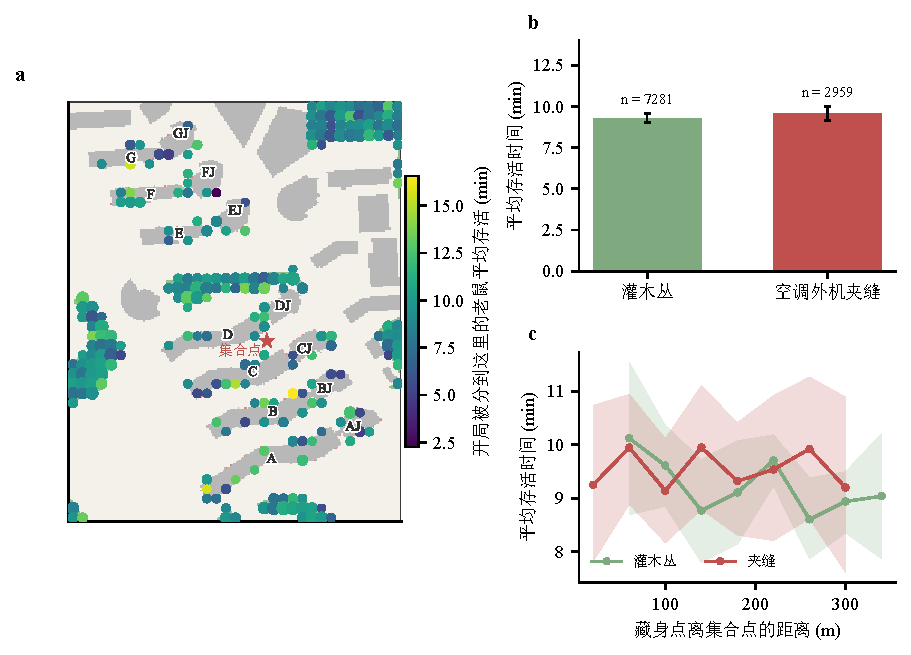
\includegraphics[width=\textwidth]{fig4_where_to_hide.pdf}
  \caption{\figlead{一旦被分到藏身点，灌木和夹缝一样安全；夹缝的优势在于离每个人都近。}
  \textbf{a}，每只老鼠开局被随机分到一个藏身点。圆点是 12 m 格内老鼠的平均存活时间（只画至少 15 只老鼠的格子），点越大样本越多；红星为集合点。
  \textbf{b}，按开局目的地的类型汇总，误差棒为按局自举的 95\% 区间。
  \textbf{c}，存活时间随藏身点到集合点距离的变化（40 m 一组，只画至少 100 只老鼠的组），阴影为 95\% 区间。共 2 × 256 局、10240 只老鼠（灌木 7281 只，夹缝 2959 只），每局 30 分钟。}
  \label{fig:spot}
\end{figure}

\subsection{上下两轮之间：会从跑转向躲，也会从躲转向跑}
\label{sec:res-rounds}
先看收益（图~\ref{fig:rounds}a）。不管第一轮有多少人躲，躲者都比跑者多活 4.5–5.5 分钟：躲者的平均存活在 9.3–10.2 分钟之间，跑者在 4.7–5.0 分钟之间。也就是说，在这个模型里“躲”是严格占优的策略，复制者动态\cite{taylor1978}唯一的稳定点是“全员都躲”。两条曲线随 $x$ 的变化都很小：躲的人越多，躲者自己略差一点（10.2 → 9.3 分钟，可能是近处的好位置被占满了），跑者基本不变（4.7–5.0 分钟）。所以每只老鼠的收益主要取决于自己怎么做，几乎不取决于别人怎么做。

再看个体模仿（图~\ref{fig:rounds}b，$K=1$ 分钟）。看到别人的结果后，第二轮确实会有人从跑转向躲：第一轮躲的比例为 0.25、0.5、0.75 时，分别有 15\%、29\%、42\% 的跑者改成躲。反方向的转化也确实存在，而且不少：同样三种情况下，分别有 34\%、24\%、12\% 的躲者改成跑。原因是单局结果的随机性很大：全员都躲时，约五分之一的老鼠能撑满 30 分钟，但也有不少人一藏好就被路过的猫看见了；一个运气差的躲者看到一个运气好的跑者，就可能改成跑。两个方向相互抵消后，第二轮躲的比例只比第一轮高 0.01–0.02（例如 0.25 → 0.27）。把 $K$ 换成 3 分钟，结果几乎不变，因为单局之间的存活差距通常远大于 3 分钟。

这对实际游戏的含义是：只看一局、只看身边一个人，“躲更好”这个结论很难传开；如果第一轮结束后有人公布\textbf{平均}结果（相当于看很多人的结果），转化会快得多。

\begin{figure}[htbp]
  \centering
  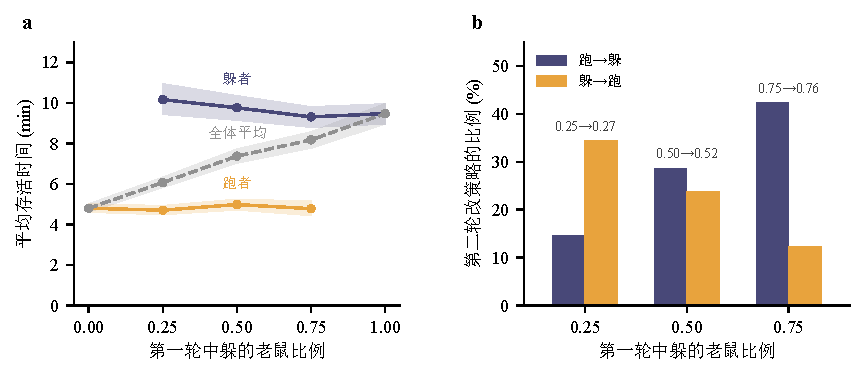
\includegraphics[width=\textwidth]{fig6_between_rounds.pdf}
  \caption{\figlead{躲在任何比例下都比跑好，但只看身边一个人的结果时，两个方向的转化都会发生，躲的比例上升得很慢。}
  \textbf{a}，第一轮中躲的比例为 $x$ 时，躲者、跑者和全体老鼠的平均存活时间（30 分钟一轮），阴影为按局自举的 95\% 区间，每个 $x$ 256 局。
  \textbf{b}，第一轮结束后每只老鼠随机看同局一个同伴，按费米模仿规则（$K=1$ 分钟）决定是否改用同伴的策略。柱是两个方向的转化比例，柱顶数字是第一轮和第二轮躲的比例。}
  \label{fig:rounds}
\end{figure}

\subsection{猫鼠共同训练：针对对手的对策，与变弱的团队}
\label{sec:res-coevo}
八组共同训练各用 3 个随机种子。训练结束后做交叉评估：除了让学出来的猫和老鼠互相对局，还让它们分别对上训练时没见过的脚本对手。只有对手固定，才能比较“谁学得更好”。每个种子评估 64 局。图~\ref{fig:coevo} 和图~\ref{fig:catreward} 中，柱高是三个种子均值的平均，黑点是各种子自己的均值，误差棒是分层自举的 95\% 区间。同组种子之间的差别往往比组间差别还大，下面的结论都只是探索性的。

\begin{figure}[htbp]
  \centering
  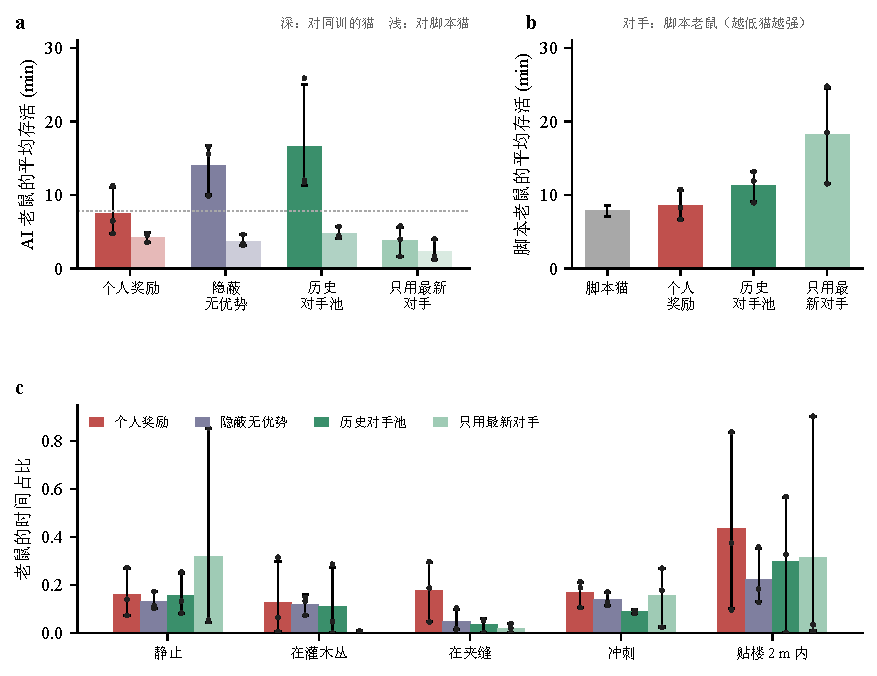
\includegraphics[width=\textwidth]{fig5_coevolution.pdf}
  \caption{\figlead{共同训练出的老鼠换成脚本猫后活得很短；历史对手池比只用最新对手好，但仍没有学到通用的躲藏。}
  \textbf{a}，各组 AI 老鼠对上一起训练的猫（深色）和对上脚本猫（浅色）时的平均存活；虚线是脚本老鼠（跑、躲各半）对脚本猫的水平。
  \textbf{b}，脚本猫与三组 AI 猫分别对上同一批脚本老鼠（跑、躲各半）时，老鼠的平均存活；存活越短，猫越强。
  \textbf{c}，AI 老鼠与一起训练的猫对局时，五类行为的时间占比（可以重叠）。
  每组 3 个种子 × 64 局，每局 30 分钟；柱高为各种子均值的平均，误差棒为分层自举（先抽种子、再抽局）的 95\% 区间，黑点为各种子的均值。}
  \label{fig:coevo}
\end{figure}

\paragraph{老鼠学会躲了吗？（RQ4）}部分学会了，但三个种子差别很大。和一起训练的猫对局时，个人奖励组的老鼠平均有 18\% 的时间待在夹缝里、16\% 的时间静止（图~\ref{fig:coevo}c）。夹缝只占可走面积的 0.2\%，老鼠却在里面待了近五分之一的时间，这不可能是随机游走的结果，是它从“多活一会儿”的奖励里自己学到的。但三个种子分别是 19\%、5\% 和 30\%，学会的程度相差很大。

\paragraph{换成没见过的对手会怎样？}个人奖励组的 AI 老鼠对上一起训练的猫，平均活 7.5 分钟；换成脚本猫以后，只剩 4.3 分钟（95\% 区间 [3.5, 4.9]），不但不如脚本躲者（11.2 分钟），连脚本跑者（5.4 分钟）都不如（图~\ref{fig:coevo}a）。团队奖励组更明显：对上一起训练的、较弱的猫能活 17.9 分钟，换成脚本猫只剩 2.1 分钟。这说明老鼠确实学到了东西，但学到的是\textbf{针对这批猫的对策}，也就是对这批猫当前策略的“最优反应”（best response），很可能利用了这批猫巡逻不系统的弱点。脚本猫会预判拦截，还会按“多久没搜过”系统地巡逻，这些对策就不灵了。双方只学会了打败对方当前的策略，这是共同训练中常见的相互过拟合。

\paragraph{和历史版本的对手对局有用吗？}有一些用，但不够。历史对手池组的老鼠对上脚本猫活 4.8 分钟（[4.1, 5.7]），只用最新对手的对照组只有 2.3 分钟（[1.2, 4.0]）；猫也一样，对上脚本老鼠时，对手池组的猫让老鼠活 11.3 分钟，对照组是 18.3 分钟，后者明显更弱（图~\ref{fig:coevo}a、b）。两组的样本量和训练轮数完全相同，差别只在对手是否多样，在本文的 3 个种子里，多样对手组在两个方向上都好于对照组，初步表明在相同的训练方式下，多样的对手有助于双方学得更通用；但样本量太小，还不能作确定性的结论。对照组的一个种子甚至退化成老鼠 85\% 的时间站着不动、猫一出现就被抓。但和普通的个人奖励组（同样的样本量，只是不分两半）相比，对手池组的老鼠只多活 0.5 分钟，区间重叠；猫还更弱一些（11.3 分钟对 8.6 分钟）。也就是说，“一半局训练老鼠、一半局训练猫”这种做法本身就有代价，对手池只是把这部分代价补了回来，AI 老鼠离脚本躲者的 11.2 分钟还差得远。要学到真正通用的躲藏本领，可能需要更大的对手池、更长的训练，或者直接把脚本猫也放进对手池。

\paragraph{藏身处没有隐蔽优势时，老鼠会不会都改成跑？}不会，它主要是不再往夹缝里躲。隐蔽无优势组的老鼠在夹缝里的时间只有 5\%（三个种子 2\%、10\%、2\%），个人奖励组是 18\%；静止（13\% 对 16\%）和冲刺（14\% 对 17\%）两组差不多，冲刺并没有增加。这和脚本实验一致：两种隐蔽优势都取消以后，躲不再比跑好（+0.3 分钟，区间包含 0），夹缝也就失去了吸引力；但冲刺会耗尽体力，所以也不会一直跑。这一组的老鼠对上脚本猫活 3.7 分钟，与同一世界里脚本老鼠的 3.6–4.3 分钟相当（表~\ref{tab:campus}“两者都无优势”一行）。

\begin{figure}[htbp]
  \centering
  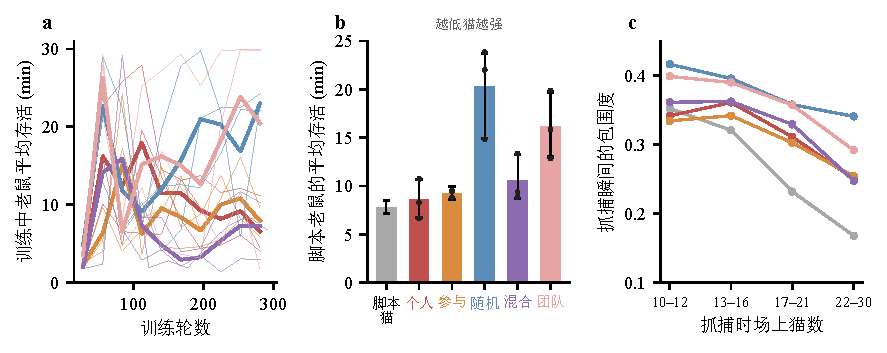
\includegraphics[width=\textwidth]{fig7_cat_reward.pdf}
  \caption{\figlead{团队平分奖励的猫明显更弱；把功劳只分给在场的猫，猫的强度回到个人奖励的水平，而把同样多的功劳随机分给几只猫，猫反而最弱。}
  \textbf{a}，训练中老鼠的平均存活（每点为一批完整对局的平均）。细线是各种子，粗线是三个种子的平均，颜色同 \textbf{b} 的横轴标签。
  \textbf{b}，脚本猫与五种奖励下的 AI 猫分别对上同一批脚本老鼠（跑、躲各半）时，老鼠的平均存活；存活越短，猫越强。“参与”即按参与分配，“随机”即随机分配。误差棒与黑点同图~\ref{fig:coevo}。
  \textbf{c}，对上脚本老鼠时，按抓捕时场上猫数分组的平均包围度（三个种子的抓捕合并计算）。}
  \label{fig:catreward}
\end{figure}

\paragraph{猫的奖励方式有影响吗？（RQ5）}有，而且是本文强化学习部分最清楚的一个结果。对上同一批脚本老鼠，个人奖励的 AI 猫让老鼠活 8.6 分钟，已经接近脚本猫的 7.8 分钟；团队平分奖励的猫则弱得多，老鼠能活 16.2 分钟（[12.9, 19.7]），三个种子（12.9、19.9、15.9 分钟）都比个人奖励的三个种子（6.7、8.3、10.7 分钟）差（图~\ref{fig:catreward}b）。其中一个团队奖励种子在和自己的老鼠对局时几乎不再抓人，老鼠平均活 29.5 分钟。

一个可能的解释是信用分配：全队平分奖励时，一只猫拿到的奖励和它自己做了什么关系很小，学习信号被大大稀释\cite{sunehag2018}。为了检验这一点，本文加了三组。\textbf{按参与分配}只把功劳分给抓捕瞬间在 15 m 以内的猫，它让老鼠活 9.3 分钟（[8.6, 10.0]），与个人奖励相当；\textbf{混合奖励}一半个人、一半平分，结果介于两者之间（10.5 分钟）。但“按参与分配”同时改了两件事：分到功劳的猫变少了，而且分到的是在场的猫。\textbf{随机分配}对照把这两件事分开：每次分给几只猫和“按参与分配”完全一样，只是随机挑。结果这组猫最弱，老鼠能活 20.3 分钟（[15.1, 23.8]），三个种子（14.9、22.0、23.9 分钟）都远差于“按参与分配”的三个种子（9.5、9.5、8.8 分钟），也不比团队平分好。也就是说，光让奖励更集中没有用；起作用的是奖励要落到真正出了力的猫身上。随机分配甚至比团队平分更差，原因可能是：两者给每只猫的期望奖励差不多，但随机分配的噪声更大，一只猫拿到的奖励和它做了什么几乎完全无关。这组对照给信用稀释的解释提供了比较直接的支持。不过“按参与分配”只是局部共享奖励，不是精确衡量每只猫贡献的差分奖励，而且每组只有 3 个种子，这个结论仍是探索性的。

团队奖励也没有让猫更会围捕。按抓捕时场上猫的数量分组后（图~\ref{fig:catreward}c），五种 AI 猫在猫多时都比脚本猫更聚集：场上 22–30 只猫时，脚本猫的包围度是 0.17，AI 猫在 0.25–0.34 之间。团队奖励和随机分配的猫包围度最高，比个人奖励高 0.03–0.09；但它们每局只抓到 11.1 只和 7.3 只，个人奖励的猫抓到 16.6 只。所以奖励与个体行为脱钩的猫更爱扎堆，抓得却更少：抓捕瞬间的聚集不等于更有效的合作，扎堆反而可能让搜索的范围变小。RQ5 的回答是：不把围捕写进规则，AI 猫在抓捕时会比脚本猫更聚集；但团队平分奖励换来的只是更多扎堆，而不是更多抓捕。真实游戏里“抓得最多的猫有奖”是个人奖励，从学习的角度看，它反而给了每只猫更清晰的信号。


% =====================================================================
\section{总结与思考}
% =====================================================================
\subsection{主要结论}
下面按五个研究问题逐一回答。所有结论都只针对本文的地图、发现模型和策略设置。

\textbf{RQ1（机制）。}在 A–G 楼这片校园里，躲确实比跑活得久：一轮 30 分钟里，就近躲进灌木或夹缝平均活 11.2 分钟，跑只活 5.4 分钟。反事实对照表明，这个优势主要来自“藏身处本身更难被看见”：只取消地形的隐蔽优势，躲的优势从 5.8 分钟降到 0.6 分钟；两种隐蔽优势都取消，就只剩 0.3 分钟，区间包含 0。只取消“站着不动更难被发现”这一项，躲仍多活 3.7 分钟。

\textbf{RQ2（最好的藏身点）。}就近选点时，夹缝最好（11.1 分钟，与“躲”相当），只躲灌木（6.3 分钟）反而不如原地不动（8.5 分钟）。但如果直接把老鼠分到藏身点，灌木和夹缝差不多一样安全（9.3 和 9.6 分钟，差别不显著）。所以好的藏身点要“藏得住、走得到”：夹缝紧贴每栋楼，走过去不用穿过大片空地。这与实战中鼠王躲在夹缝里、一直没被抓到的经验一致。

\textbf{RQ3（上下两轮之间的转化）。}不管第一轮有多少人躲，躲都比跑多活 4.5–5.5 分钟，是严格占优的策略。但如果每个人只看身边一个人的结果，两个方向的转化都会发生：第一轮四分之一的人躲时，15\% 的跑者改成躲，同时 34\% 的躲者改成跑。单局结果的运气成分很大，第二轮躲的比例只上升 0.01–0.02。

\textbf{RQ4（老鼠的学习）。}只奖励“活得久”的 AI 老鼠，部分学会了躲进夹缝、站着不动，但三个种子差别很大。它学到的是针对一起训练的猫的对策：换成脚本猫后，个人奖励组的 AI 老鼠只活 4.3 分钟，还不如脚本跑者。和历史版本的对手对局，比只和最新对手对局学得更通用（对上脚本猫 4.8 分钟对 2.3 分钟），但仍远不如脚本躲者。取消隐蔽优势后，AI 老鼠几乎不再进夹缝（18\% → 5\%），但冲刺没有增加，也没有变成“只会跑”。

\textbf{RQ5（猫的学习）。}团队平分奖励让猫明显变弱：脚本老鼠对上它能活 16.2 分钟，对上个人奖励的猫只活 8.6 分钟，三个种子无一例外。把功劳只分给抓捕时在场的猫，猫的强度就回到个人奖励的水平（9.3 分钟）；而把同样多的功劳随机分给几只猫，猫反而最弱（20.3 分钟）。所以起作用的不是奖励更集中，而是奖励落到了真正出力的猫身上，这支持“平分稀释了学习信号”的解释。不把围捕写进规则，AI 猫在抓捕时比脚本猫更聚集；团队奖励的猫最爱扎堆，抓得却最少。

\subsection{博弈论视角的思考}
这个游戏里有两层博弈。猫和老鼠之间，一开始是搜索博弈，一旦被发现就变成追逃博弈：“躲”把博弈尽量留在搜索阶段，“跑”则让自己更早进入追逃阶段。在体力有限、猫越来越多的条件下，追逃阶段对老鼠越来越不利，这就是“躲”占优的原因，而藏身处的隐蔽性决定了这个优势有多大。

老鼠和老鼠之间，被抓即转化在原理上带来外部性：每只老鼠被抓，其余老鼠就多一个敌人。但在本文的数值里，这种外部性很弱，每只老鼠的收益主要取决于自己选躲还是选跑，和别人怎么选关系不大。所以这里并不像公地悲剧那样“个人理性导致集体受损”：对个人最好的选择（躲）恰好也是对集体最好的选择。在本文的模仿模型里，真正阻碍“全员都躲”的是学习过程的局限：只看一局、只看一个人，运气会掩盖策略之间的真实差距。

猫的奖励设计可以类比机制设计中的激励结构：组织者通过奖励规则影响参与者的行为。不过，机制设计假设参与者是理性的，而本文的猫是靠强化学习去适应奖励的；团队奖励变弱的原因不是博弈论意义上的搭便车，而是学习信号被稀释。从博弈的角度看，团队奖励似乎更鼓励合作；但在学习意义上，奖励需要能追溯到个体的行为才有用。现实中“抓得最多的猫有奖”恰好给了每只猫清晰的激励。

\subsection{方法上的迭代与局限}
小场地阶段，AI 老鼠先后找到了两个环境漏洞：一是猫的巡逻点到不了墙角，老鼠就躲在角落里不动；二是猫只会直线追，老鼠绕着跑就能甩掉。给猫加上搜索记忆和预判拦截之后，结论才稳定下来。这说明对手太弱时，学到的“策略”可能只是漏洞。

本文还有几处局限。第一，发现概率的系数来自游戏体验，不是测量值；反事实对照说明了结论依赖哪一项，但具体的存活分钟数不能当真。第二，地图有一部分是合成的：OSM 是二维地图，没有空调外机的数据，空调外机是按固定随机种子沿外墙放置的；灌木丛来自 OSM 的林地和行道树，也不完全等于实地。第三，强化学习的规模有限：每组只有 3 个种子、300 轮（对手池两组 600 轮），同组种子之间差别很大，所以强化学习部分的比较都是探索性的。对手池组有两个模型训练中途中断过一次（一次是显卡驱动重置，一次是某一批只有一个有效样本、标准化时出现数值错误），都从最近的检查点“热重启”，环境和随机数状态没有恢复。第四，“按参与分配”只是局部共享奖励，不是精确衡量个体贡献的差分奖励；随机分配对照虽然支持信用稀释的解释，但每组只有 3 个种子，还不能算定论。第五，模拟本身还有两处近似：抓捕虽然在每个子步检查距离，但子步之间只按端点采样，斜着擦身而过的极近接触仍可能漏判；抓捕记给哪只猫、“按参与分配”的 15 m 范围和包围度，用的是这一步结束时的位置，而不是接触的那一刻，两者最多相差半秒。第六，两轮转化实验中的老鼠只有“躲”“跑”两种脚本策略，模仿规则也是假设的，真实的人还会听别人讲、会看整体结果。

下一步可以从三方面改进：用真正的差分奖励或值分解、更多的种子，确认团队奖励变弱的原因，并看能否在不削弱猫的情况下带来真正的围捕；扩大历史对手池、把脚本猫也放进对手池，看 AI 老鼠能不能学到对任何猫都管用的躲藏；回到实地标出真实的灌木与空调外机位置，再跑一次“哪里最好躲”。


% =====================================================================
\renewcommand{\refname}{\normalsize\normalfont 参考文献：}
\begin{thebibliography}{99}
\small
\setlength{\itemsep}{0pt}
\bibitem{alpern2003} Alpern S, Gal S. The theory of search games and rendezvous[M]. Boston: Kluwer Academic Publishers, 2003.
\bibitem{chung2011} Chung T H, Hollinger G A, Isler V. Search and pursuit-evasion in mobile robotics: a survey[J]. Autonomous Robots, 2011, 31(4): 299-316.
\bibitem{baker2020} Baker B, Kanitscheider I, Markov T, et al. Emergent tool use from multi-agent autocurricula[C]//International Conference on Learning Representations. 2020.
\bibitem{schulman2017ppo} Schulman J, Wolski F, Dhariwal P, et al. Proximal policy optimization algorithms[EB/OL]. arXiv preprint arXiv:1707.06347, 2017. \url{https://arxiv.org/abs/1707.06347}.
\bibitem{schulman2016gae} Schulman J, Moritz P, Levine S, et al. High-dimensional continuous control using generalized advantage estimation[C]//International Conference on Learning Representations. 2016.
\bibitem{yu2022mappo} Yu C, Velu A, Vinitsky E, et al. The surprising effectiveness of PPO in cooperative multi-agent games[C]//Advances in Neural Information Processing Systems. 2022, 35: 24611-24624.
\bibitem{grupen2022} Grupen N, Selman B, Lee D D. Cooperative multi-agent fairness and equivariant policies[C]//Proceedings of the AAAI Conference on Artificial Intelligence. 2022, 36(9): 9350-9359.
\bibitem{leibo2017} Leibo J Z, Zambaldi V, Lanctot M, et al. Multi-agent reinforcement learning in sequential social dilemmas[C]//Proceedings of the 16th Conference on Autonomous Agents and MultiAgent Systems. 2017: 464-473.
\bibitem{taylor1978} Taylor P D, Jonker L B. Evolutionary stable strategies and game dynamics[J]. Mathematical Biosciences, 1978, 40(1-2): 145-156.
\bibitem{szabo1998} Szabó G, Tőke C. Evolutionary prisoner's dilemma game on a square lattice[J]. Physical Review E, 1998, 58(1): 69-73.
\bibitem{traulsen2006} Traulsen A, Nowak M A, Pacheco J M. Stochastic dynamics of invasion and fixation[J]. Physical Review E, 2006, 74(1): 011909.
\bibitem{kermack1927} Kermack W O, McKendrick A G. A contribution to the mathematical theory of epidemics[J]. Proceedings of the Royal Society of London. Series A, 1927, 115(772): 700-721.
\bibitem{osm} OpenStreetMap contributors. OpenStreetMap[EB/OL]. [2026-11-05]. \url{https://www.openstreetmap.org}.
\bibitem{sunehag2018} Sunehag P, Lever G, Gruslys A, et al. Value-decomposition networks for cooperative multi-agent learning based on team reward[C]//Proceedings of the 17th International Conference on Autonomous Agents and MultiAgent Systems. 2018: 2085-2087.
\bibitem{agarwal2021} Agarwal R, Schwarzer M, Castro P S, et al. Deep reinforcement learning at the edge of the statistical precipice[C]//Advances in Neural Information Processing Systems. 2021, 34: 29304-29320.
\end{thebibliography}

\end{document}
